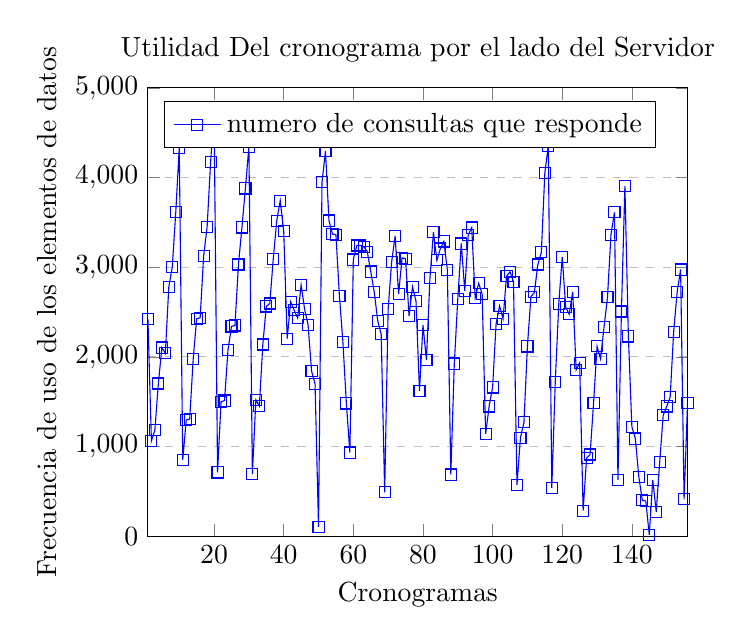
\begin{tikzpicture}
\begin{axis}[
    title={Utilidad Del cronograma por el lado del Servidor},
    xlabel={Cronogramas},
    ylabel={Frecuencia de uso de los elementos de datos},
    xmin=1, xmax=156,
    ymin=0, ymax=5000,
    xtick={},
    ytick={},
    legend pos=north west,
    ymajorgrids=true,
    grid style=dashed,
]

\addplot[
    color=blue,
    mark=square,
    ]
    coordinates {
%UTILIDAD TOTAL
(1,2419)
(2,1063)
(3,1187)
(4,1703)
(5,2104)
(6,2040)
(7,2781)
(8,3004)
(9,3616)
(10,4332)
(11,851)
(12,1295)
(13,1307)
(14,1975)
(15,2426)
(16,2435)
(17,3123)
(18,3448)
(19,4171)
(20,4736)
(21,711)
(22,1498)
(23,1513)
(24,2079)
(25,2339)
(26,2350)
(27,3030)
(28,3443)
(29,3878)
(30,4345)
(31,693)
(32,1520)
(33,1451)
(34,2138)
(35,2562)
(36,2595)
(37,3092)
(38,3518)
(39,3742)
(40,3402)
(41,2203)
(42,2615)
(43,2521)
(44,2433)
(45,2801)
(46,2531)
(47,2357)
(48,1841)
(49,1700)
(50,104)
(51,3948)
(52,4295)
(53,3520)
(54,3369)
(55,3363)
(56,2679)
(57,2167)
(58,1480)
(59,933)
(60,3085)
(61,3242)
(62,3242)
(63,3229)
(64,3174)
(65,2951)
(66,2724)
(67,2404)
(68,2252)
(69,489)
(70,2535)
(71,3057)
(72,3349)
(73,2699)
(74,3105)
(75,3094)
(76,2457)
(77,2781)
(78,2620)
(79,1618)
(80,2353)
(81,1964)
(82,2875)
(83,3390)
(84,3077)
(85,3208)
(86,3287)
(87,2971)
(88,687)
(89,1925)
(90,2647)
(91,3264)
(92,2737)
(93,3360)
(94,3442)
(95,2659)
(96,2820)
(97,2701)
(98,1141)
(99,1447)
(100,1659)
(101,2366)
(102,2568)
(103,2423)
(104,2900)
(105,2949)
(106,2838)
(107,572)
(108,1098)
(109,1269)
(110,2116)
(111,2670)
(112,2719)
(113,3030)
(114,3165)
(115,4052)
(116,4355)
(117,540)
(118,1718)
(119,2588)
(120,3116)
(121,2552)
(122,2474)
(123,2725)
(124,1856)
(125,1933)
(126,285)
(127,871)
(128,911)
(129,1486)
(130,2117)
(131,1978)
(132,2331)
(133,2666)
(134,3362)
(135,3612)
(136,629)
(137,2506)
(138,3908)
(139,2228)
(140,1221)
(141,1089)
(142,661)
(143,401)
(144,392)
(145,16)
(146,628)
(147,270)
(148,831)
(149,1347)
(150,1447)
(151,1551)
(152,2274)
(153,2721)
(154,2974)
(155,411)
(156,1489)
(157,990)
    };
    \legend{numero de consultas que responde}

\end{axis}
\end{tikzpicture}

